% !TEX root = tracking.tex
\subsection{10D quadrotor-3D single integrator example with RRT\label{sec:resultsRRT}}

Our second example involves a 10D near-hover quadrotor developed in \cite{Bouffard12} as the tracking model and a single integrator in 3D space as planning model.
Planning is done using RRT, a well-known sampling-based planner that quickly produces geometric paths from a starting position to a goal position \cite{Kuffner2000,Kavraki1996}.
Paths given by the RRT planner is converted to time-stamped trajectories by placing a maximum velocity in each dimension along the generated geometric paths.

The dynamics of tracking model and of the 3D single integrator is as follows:

\begin{equation}
\label{eq:Quad10D_dyn}
\begin{bmatrix}
\dot{x}\\
\dot{v_x}\\
\dot{\theta_x}\\
\dot\omega_x\\
\dot{y}\\
\dot{v_y}\\
\dot{\theta_y}\\
\dot\omega_y\\
\dot{z}\\
\dot{v_z}
\end{bmatrix}
=
\begin{bmatrix}
v_x + d_x\\
g \tan \theta_x\\
-d_1 \theta_x + \omega_x\\
-d_0 \theta_x + n_0 a_x\\
v_y + d_y\\
g \tan \theta_y\\
-d_1 \theta_y + \omega_y\\
-d_0 \theta_y + n_0 a_y\\
v_z + d_z\\
k_T a_z - g
\end{bmatrix}, \quad
\begin{bmatrix}
\dot{\hat x}\\
\dot{\hat y}\\
\dot{\hat z}\\
\end{bmatrix} =
\begin{bmatrix}
\hat v_x \\
\hat v_y \\
\hat v_z
\end{bmatrix},
\end{equation}
\noindent where quadrotor states $(x, y, z)$ denote the position, $(v_x, v_y, v_z)$ denote the velocity, $(\theta_x, \theta_y)$ denote the pitch and roll, and $(\omega_x, \omega_y)$ denote the pitch and roll rates. 
The controls of the 10D system are $(u_x, u_y, u_z)$, where $u_x$ and $u_y$ represent the desired pitch and roll angle, and $u_z$ represents the vertical thrust.

The 3D system controls are $(\hat v_x, \hat v_y, \hat v_z)$, and represent the velocity in each positional dimension. 
The disturbances in the 10D system $(\dstb_x, \dstb_y, \dstb_z)$ are caused by wind, which acts on the velocity in each dimension. 

The model parameters are chosen to be $d_0=10$, $d_1=8$, $n_0=10$, $k_T=0.91$, $g=9.81$, $|u_x| |u_y| \le \pi/9$, $u_z \in [0, 1.5g]$, $|\hat v_x|, |\hat v_y|, |\hat v_z| \le 0.5$.
The disturbance bounds were chosen to be $|d_x|, |d_y|, |d_z| \le 0.1$.

\subsubsection{Offline computation}
We define the relative system states to consist of the error states, or relative position $(x_r, y_r, z_r)$, concatenated with the rest of the state variables of the 10D quadrotor model.
Defining $\rtrans = \mathbf I_{10}$ and 

\begin{equation*}
\ptmat = 
\begin{bmatrix}
  \begin{bmatrix} 1 \\ \mathbf 0_{3 \times 1} \end{bmatrix} 
    & \mathbf 0_{4\times 1} 
    & \mathbf 0_{4\times 1} \\
  \mathbf 0_{4\times 1} 
    & \begin{bmatrix} 1 \\ \mathbf 0_{3 \times 1} \end{bmatrix} 
    &  \mathbf 0_{4\times 1} \\
  \mathbf 0_{2\times 1} 
    & \mathbf 0_{2\times 1} 
    & \begin{bmatrix} 1 \\ 0 \end{bmatrix}
\end{bmatrix},
\end{equation*}

\noindent we obtain the following relative system dynamics:

\begin{equation}
\label{eq:Quad10DRel_dyn}
\begin{bmatrix}
\dot x_r\\
\dot v_x\\
\dot \theta_x\\
\dot\omega_x\\
\dot y_r\\
\dot v_y\\
\dot \theta_y\\
\dot\omega_y\\
\dot z_r\\
\dot v_z
\end{bmatrix} =
\begin{bmatrix}
v_x - \hat v_x + d_x\\
g \tan \theta_x\\
-d_1 \theta_x + \omega_x\\
-d_0 \theta_x + n_0 u_x\\
v_y - \hat v_y + d_y\\
g \tan \theta_y\\
-d_1 \theta_y + \omega_y\\
-d_0 \theta_y + n_0 u_y\\
v_z - \hat v_z + d_z\\
k_T u_z - g
\end{bmatrix}.
\end{equation}


The relative system dynamics given in \eqref{eq:Quad10DRel_dyn} is decomposable into three independent subsystems involving the sets of variables $(x_r, v_x, \theta_x, \omega_x)$, $(x_y, v_y, \theta_y, \omega_y)$, $(z_r, v_z)$, allowing us to choose the error function to be also in the decomposable form of $\errfunc(\rstate) = \max(x_r^2, y_r^2, z_r^2)$, so that we can solve \eqref{eq:HJVI} tractably since each subsystem is at most 4D \cite{Chen2016DecouplingJournal}. 

The left subplot of Fig. \ref{fig:valfuncRRT} shows the the projection of the value function $\valfunc$ onto the $(x_r, v_x)$ space resulting from solving \eqref{eq:HJVI} over an increasingly long time horizon.
Starting from $\tau=0$, we have that $\errfunc(\rstate) = \valfunc(\rstate, 0)$.
As $\tau$ increases, the value function evolves according to \eqref{eq:HJVI}, and eventually converges when $\tau$ reaches $3.5$.
This implies that $\valfunc_\infty(\rstate) = \valfunc(\rstate, \tau=3.5)$, since we would still obtain the same function even if we let $\tau$ approach infinity.
The horizontal plane shows the minimum value, $\underline\valfunc = 0.3$, which corresponds to a TEB of approximately 0.55.

The right subplot of Fig. \ref{fig:valfuncRRT} shows the $\underline\valfunc = 0.3$ level set of value function projection, which is the projection, onto the $(x_r, v_x)$ space, of the TEB $\TEB_{\estate, \infty}$ according to \eqref{eq:TEBp:inf}.
The range of $x_r$ provides the TEB used for the planner, $\TEB_{\pstate, \infty}$, as given in \eqref{eq:TEBp:inf}.

The value function and TEB in the $(y_r, v_y, \theta_y, \omega_y)$ and $(z_r, v_z)$ spaces are combined together to form the TEB in 3D positional space.
For conciseness, these value functions are not shown; however, one can see the resulting TEB in Fig. \ref{fig:simRRT} and \ref{fig:simRRT_combined} as the translucent red box.

Offline computations were done on a laptop with an Intel Core i7 4702HQ CPU using a MATLAB implementation of level set methods \cite{Mitchell07c} used for solving \eqref{eq:HJVI}.
The 4D computations were done on a $61\times 61 \times 41 \times 41$ grid, took approximately 12 hours, and required approximately 300 MB of RAM.
The 2D computation in the $(z_r, v_z)$ space was done on a $101 \times 101$ grid, took approximately 15 seconds, and required negligible RAM.

\begin{figure}
  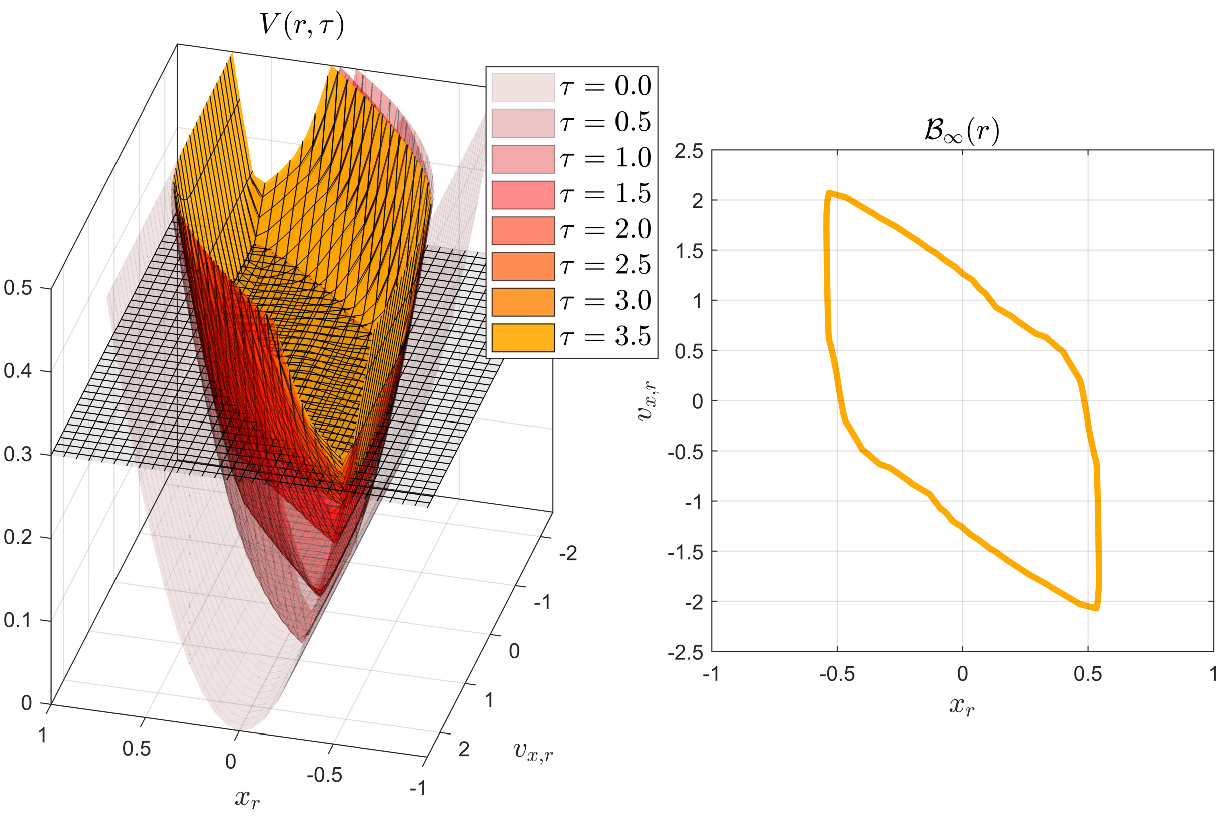
\includegraphics[width=\columnwidth]{fig/Q10D_Q3D/valfunc}
  \caption{}
  \label{fig:valfuncRRT}
\end{figure}

\subsubsection{Online sensing and planning}
The simulation involving the 10D quadrotor model tracking the 3D single integrator is shown in Fig. \ref{fig:simRRT} and \ref{fig:simRRT_combined}.
Here, the system aims to start at $(x,y,z) = (-12, 0, 0)$ and reach $(12, 0, 0)$. 
Three rectangular obstacles, which make up the constraints $\constr$, are present and initially unknown.
Before the obstacles are sensed by the system, they are shown in gray, and when the tracking system is within 1.5 units away from a part of an obstacle, that part is revealed to the system as the sensed obstacles which form the sensed constraints $\constrSense$.
The sensed obstacles are colored red.
Whenever new obstacles are revealed, the planning system replans using RRT, in real time, a trajectory to the goal while avoiding the augmented constraint set $\constrAug$.

Fig. \ref{fig:simRRT} shows the entire trajectory, with the end of the trajectory being close to the goal position.
The planning system state is shown as a small green star, and the translucent box around it depicts the TEB: the tracking system position is guaranteed to reside within this box.
Therefore, as long as the planning system plans in a way such that the the TEB does not intersect with the obstacles, the tracking system is guaranteed to be safe.
Due to the random nature of RRT, during the simulation the system appears to randomly explore to look for an unobstructed path to the obstacle; we did not implement any exploration algorithms.

Fig. \ref{fig:simRRT_combined} shows three different time snapshots of the simulation.
At $t=8$, the planning system has sensed a portion of the previously unknown obstacles, and replans, so that the path deviates from a straight line from the initial position to the goal position.
The subplot showing $t = 47.7$ is rotated to show the trajectory up to this time from a more informative view angle.
Here, the tracking system has safely passed by the first planar obstacle, and is moving around the second. 
Note that the TEB never intersects the obstacles, implying that the tracking system is guaranteed to avoid collision with the obstacles, since it is guaranteed to stay within the TEB.
At $t=83.5$, the tracking system safely passes by the last planar obstacle.

\begin{figure}
  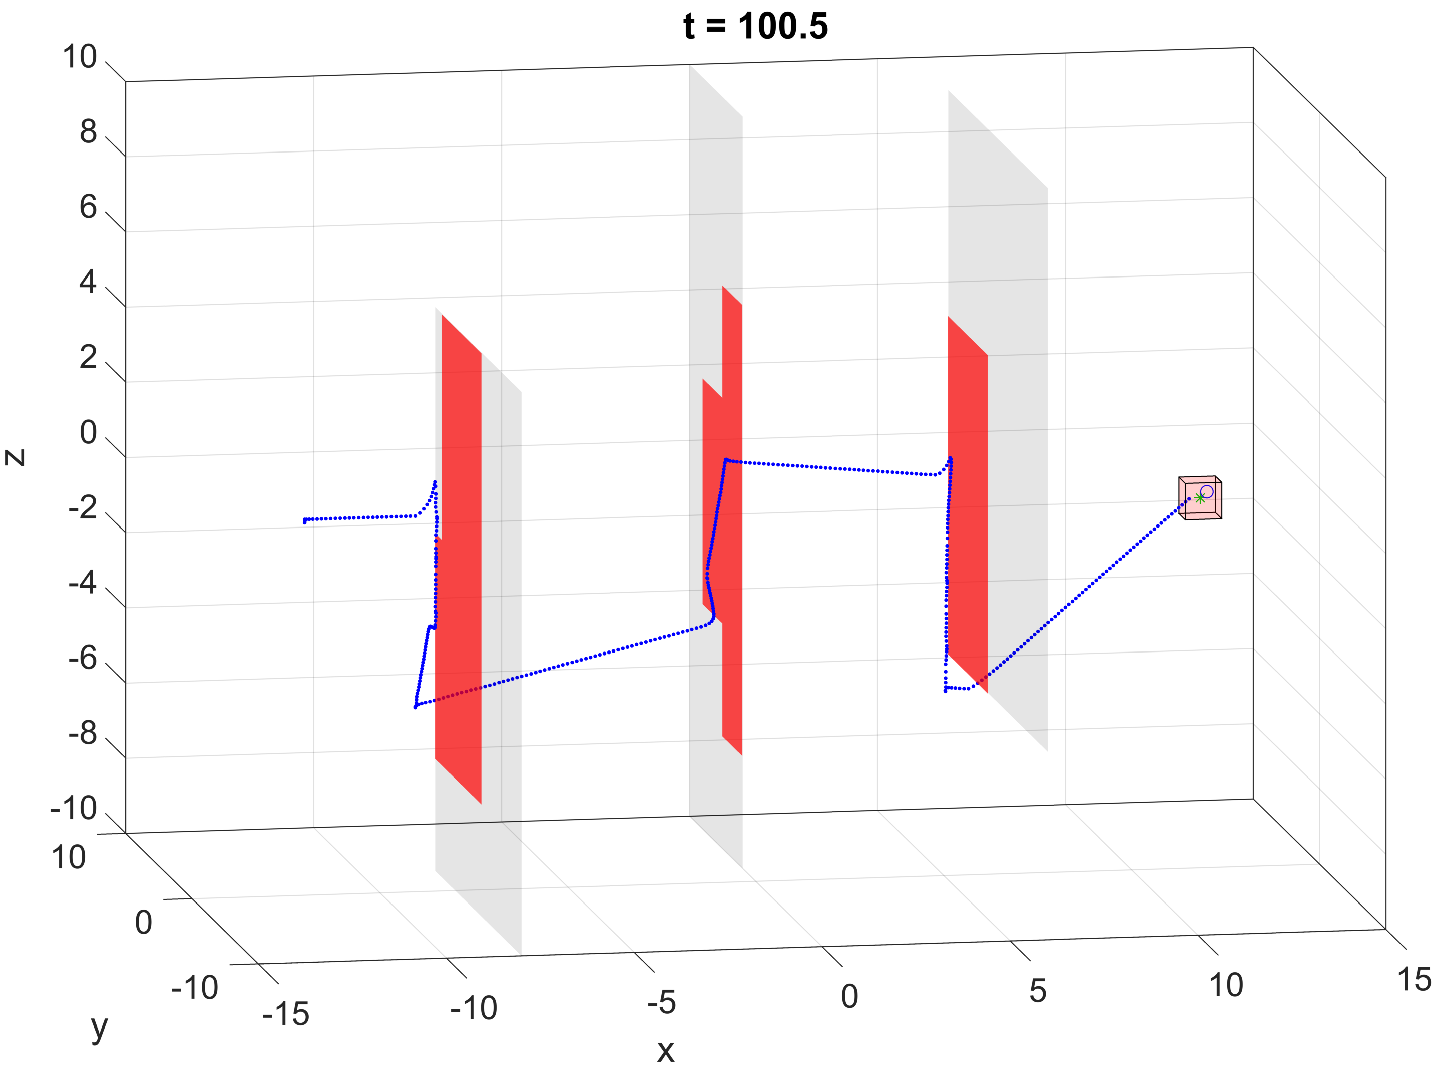
\includegraphics[width=\columnwidth]{fig/Q10D_Q3D/10050}
  \caption{Simulation of the 10D quadrotor tracking (trajectory shown in blue) a 3D single integrator (position shown as green star inside red box) in order to perform real-time robust planning. The system senses initially unknown obstacles (gray), which are revealed (revealed parts shown in red) as the system approaches them. Replanning is done in real-time by RRT when new obstacles are sensed. The TEB is shown as the red box, and is the set of positions that the 10D quadrotor is guaranteed to remain within.}
  \label{fig:simRRT}
\end{figure}

\begin{figure}
  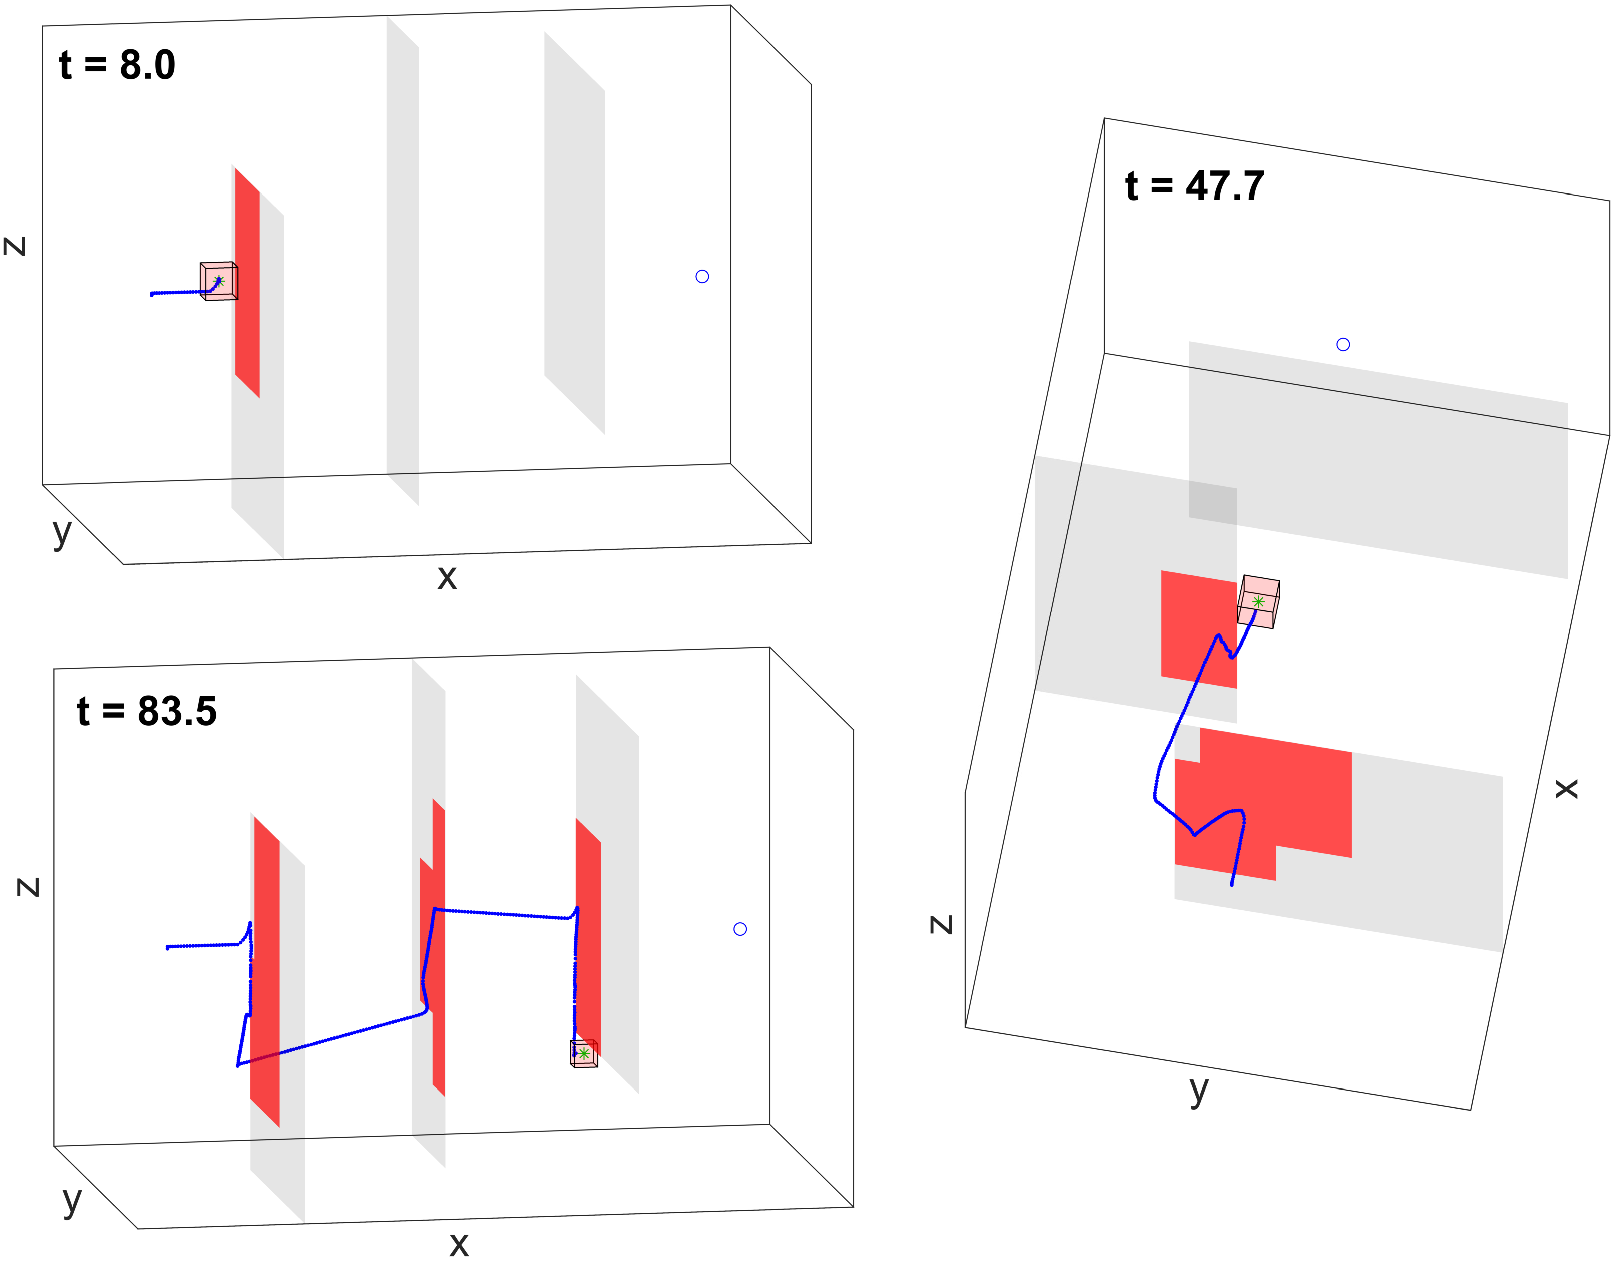
\includegraphics[width=\columnwidth]{fig/Q10D_Q3D/combined}
  \caption{Three time snapshots of the simulation in Fig. \ref{fig:simRRT}.}
  \label{fig:simRRT_combined}  
\end{figure}

Fig. \ref{fig:tracking_error_RRT} shows the maximum tracking error, in the three positional dimensions over time.
The red points indicate the time points at which the optimal tracking controller from Eq. \eqref{eq:opt_ctrl_inf} was used; this is the safety controller depicted in Fig. \ref{fig:hybrid_ctrl}. 
The blue points indicate the time points at which a performance controller, also depicted in Fig. \ref{fig:hybrid_ctrl}, was used.
For the performance controller, we used a simple proportional controller that depends on the tracking error in each positional dimension; this controller is used whenever the tracking error is less than a quarter of the TEB.
From Fig. \ref{fig:tracking_error_RRT}, one can observe that the tracking error is always less than the TEB implied by the value function.
The disturbance was chosen to be uniformly random within the chosen bounds.


\begin{figure}
  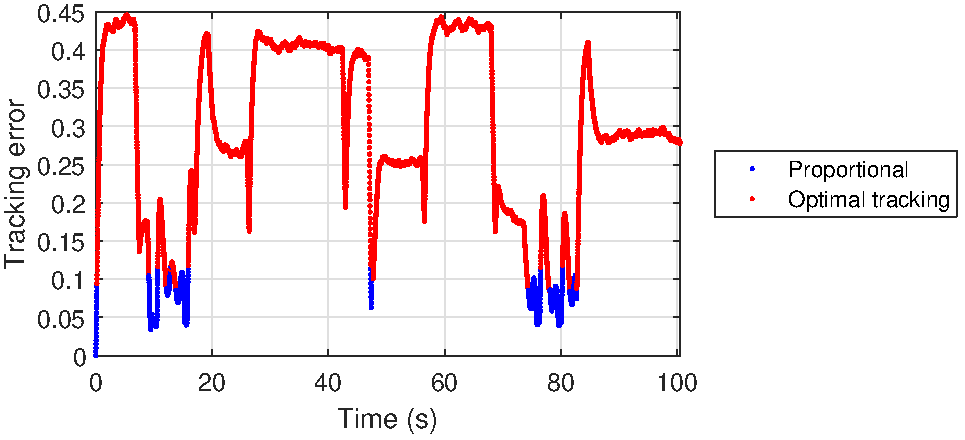
\includegraphics[width=\columnwidth]{fig/Q10D_Q3D/tracking_error}
  \caption{Tracking error over time for the 10D-3D example. The red dots indicate that the optimal tracking controller in \eqref{eq:opt_ctrl_inf} is used, while the blue dots indicate that an LQR controller for the linearized system is used. The tracking error stays well below the predicted TEB of 0.55.}
  \label{fig:tracking_error_RRT}  
\end{figure}

The simulation was done in MATLAB on a desktop computer with an Intel Core i7 2600K CPU.
The time was discretized in increments of 0.01.
Per iteration, planning with RRT using a simple multi-tree RRT planner implemented in MATLAB modified from \cite{Gavin2013} took on average 5 ms, and computing the tracking controller took on average 5.5 ms. 

